\section{Amplifier Circuits}
\textit{Amplifiers circuits} \cite{amplifier-circuit} are circuits which increase
an electrical input signal according to a specific transformation function (gain)
for each different topology. The circuit for small input signals is normally
composed by an operational amplifier, resistors, trimmer potentiometers to adjust
the gain and capacitors for frequency filtering.\\
It was required by the project an amplifier with a gain of at least 1000, beacuse, as it was
mentioned on \autoref{pickup} the tested output coil presented the value around 0.1 mV and the
circuit needs a signal of around 1V to work as expected on the AD converter, that can be powered by a sigle 5V supply, provided by the USB port. The circuit
should be cheap (and thus compact) when compared to the existent systems which usually need
multiple complex modules to perform the same action as the proposed in this project. \\
It was researched some types of amplifiers circuits in \citeonline{Milmann}
and in \citeonline{OpAmps}. After verifying some amplifier topologies it was
selected two different circuits which attend to this project's requirements.
The first circuit uses the Texas Instruments INA 326 Instrumental Amplifier.% and the
%second uses the Texas Instruments TLV 4316 Operational Amplifier.
This topology
can be supplied with a single 5V source and can reach the desirable gain without
distortion on the desired frequency range (human audible frequencies) with a single
amplifier per channel.\\

\subsection{INA 326 Project}
The project using the INA 326 IC started by researching the \textit{component datasheet}
\cite{INA326} and the \textit{supplier catalogue} \cite{OpAmps}. In these documents
it was verified the circuit topology \autoref{INA_topology} which provides the
desired gain for the pickup signal respecting this project's initial requests.\\
This recommended circuit's gain is obtained by \autoref{INA_Gain} which is
provided by the \textit{component datasheet} \cite{INA326}:

\begin{equation}
  \label{INA_Gain}
  G=2*\frac{(R_2||R_2 ')}{R_1}
\end{equation}

Both the $R_0$ resistor and the $C_0$ capacitor were excluded because they were not
relevant for our requirements. The values for the remaining components were calculated
and the circuit was build to test it's results for the desired application.
After verifying the circuit does work properly, giving the desirable value on the output and without
distortions on single supply method, the schematic \autoref{INA-single-channel-schematic} was
developed using the software CadSoft Eagle Professional 7.6.0.
\begin{figure}[!htpb]
  \centering
  \caption{INA 326 topology}
  \label{INA_topology}
  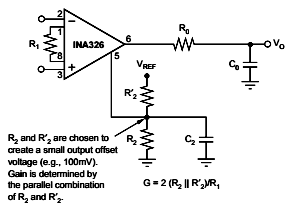
\includegraphics[scale=0.7]{images/INA/datasheet}
  \legend{Source: \citeonline{INA326}}
\end{figure}

\begin{figure}[!htpb]
  \centering
  \caption{INA 326 Schematic Circuit}
  \label{INA-single-channel-schematic}
  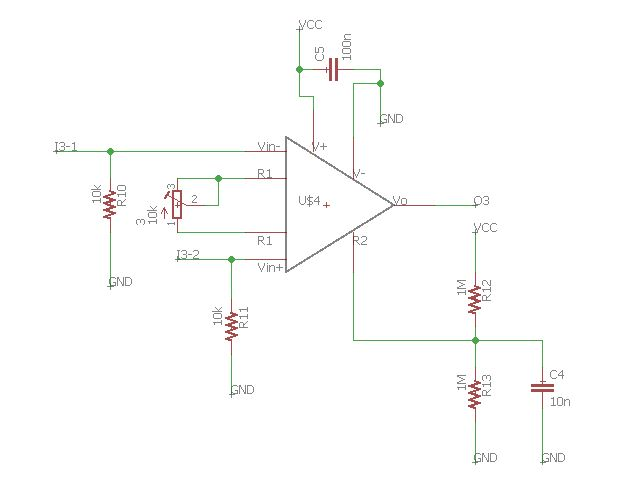
\includegraphics[scale=0.65]{images/INA/single-channel-schematic}
  \legend{Source: Authors}
\end{figure}
TODO -> INCREASE RESOLUTION OF \autoref{INA-single-channel-schematic}\\

It was decided to use trimmer potentiometers on the amplification circuit to
regulate the gain for each channel. The desired gain range was achieved by selecting
the component values showed at \autoref{INA-single-channel-schematic}. The complete
schematic is just a replication of \autoref{INA-single-channel-schematic}
for each channel, and can be seen at \autoref{INA-complete-schematic}.\\
A PCB was then built, using the same software described on the schematic modeling, resulting
in the board seen at \autoref{INA-PCB}. It has two layers, with track width of 15 mils.
It was assembled on FR4 dual layer copper board, using both through-hole and
surface-mount technologies. This choice was made due the facility of the assembly
of the through-hole components and the availability of the IC only in surface (SOP-8)
encapsulation. The generated gerber files were sent to an internal manufacturer
at UTFPR, which gave the board seen at \autoref{INA-printed}.\\
The component list for this board is as in \autoref{INA-BOM}.
\begin{table}[htb]
  \begin{center}
    \ABNTEXreducedfont
    \caption[INA Board BOM]{INA Board BOM}
    \label{INA-BOM}
    \begin{tabular}{c|c|c}
      \hline
      Name & Quantity & Value\\
      \hline \hline
      INA 326 & 6 & \\
      Trimmer Potentiometer & 6 & 10k$\Omega$ \\
      Ceramic Capacitor & 6 & 10nF \\
      Electrolytic Capacitor & 6 & 100nF x 50V \\
      Resistor & 12 & 10k$\Omega$ \\
      Resistor & 12 & 1M$\Omega$ \\
      Pin bar & 1 & 6 positions  \\
      Pin bar & 1 & 12 positions dual track \\
      Pin bar & 1 & 2 positions \\
      \hline
    \end{tabular}
    \legend{Source: authors}
  \end{center}
\end{table}

\begin{figure}[!htpb]
  \centering
  \caption{Projected INA PCB}
  \label{INA-PCB}
  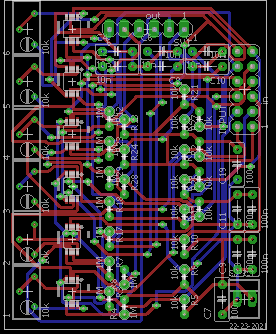
\includegraphics[scale=1.5]{images/INA/PCB}
  \legend{Source: Authors}
\end{figure}

\begin{figure}[!htpb]
  \centering
  \caption{PCB Project}
  \label{INA-printed}
  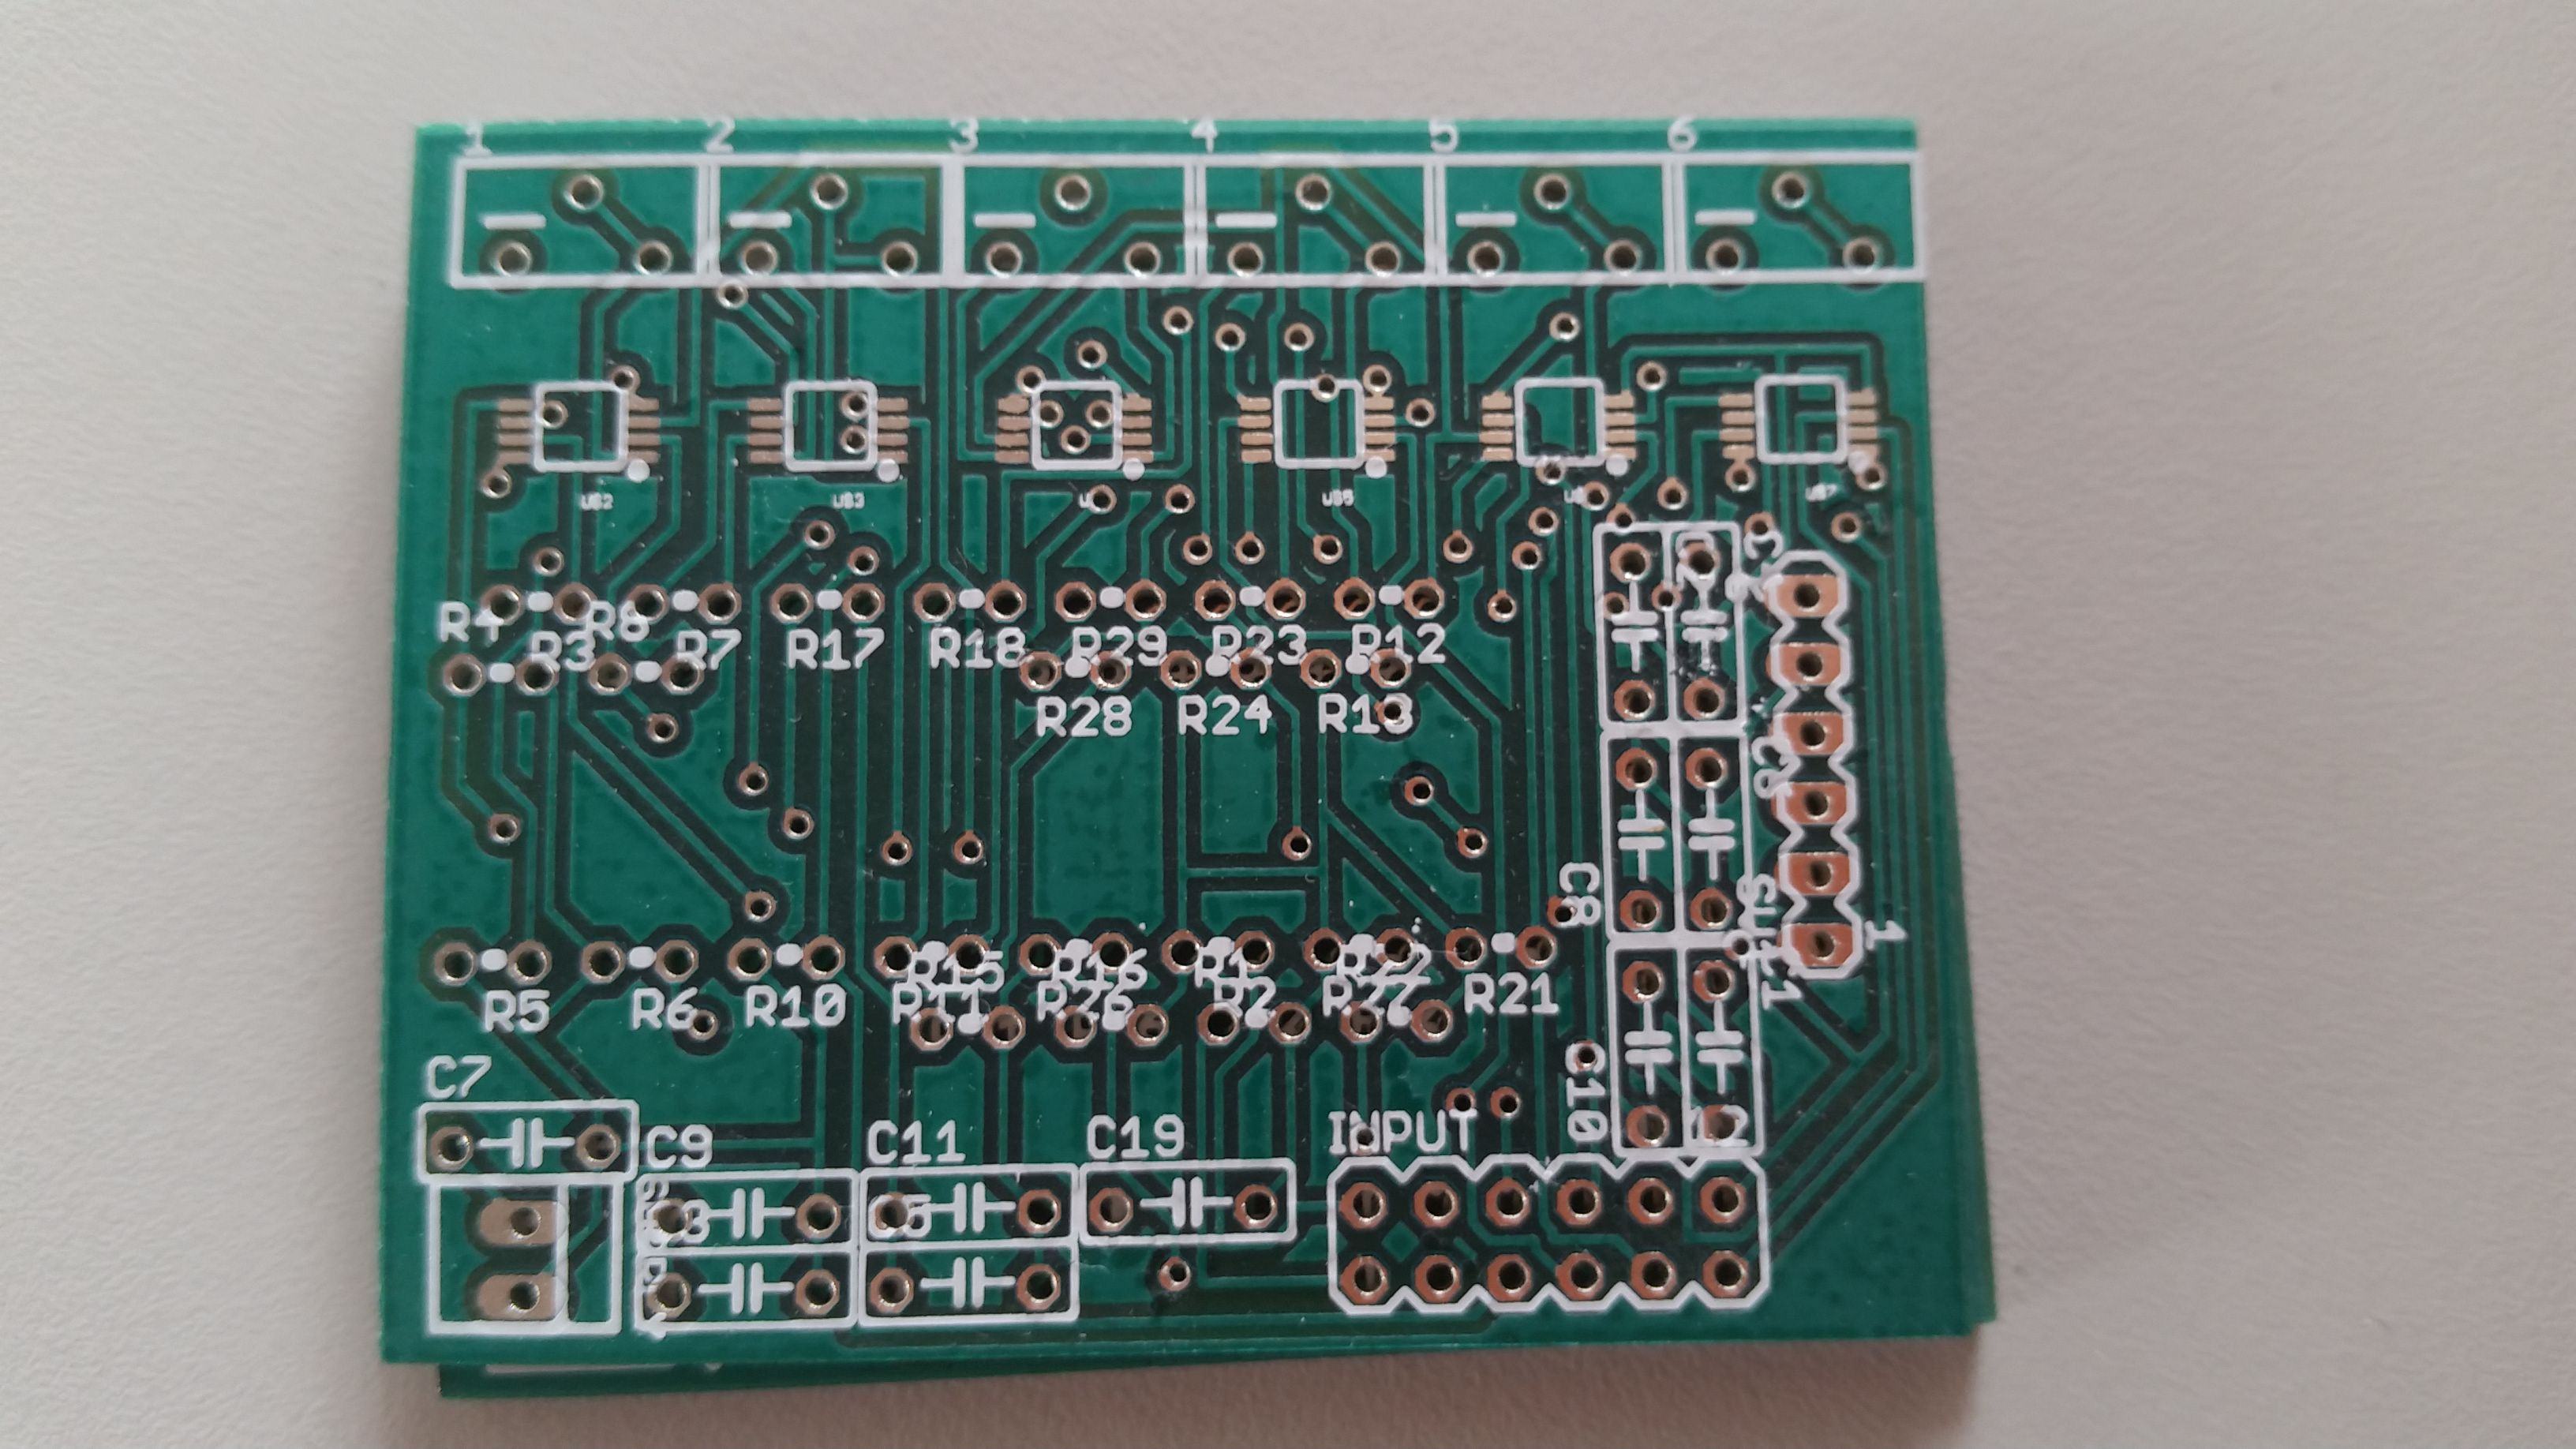
\includegraphics[scale=0.08]{images/INA/printed.jpeg}
  \legend{Source: Authors}
\end{figure}
After soldering all the components it was performed some bench tests to verify the
functionality of the amplifier circuit. The result showed that the circuit attends
the required functionality, amplifying the signal from a peak-to-peak of about 1mV
to 1.5V for the entire range of audible frequencies, proving that the circuit is
working perfectly and attending the demands of the project. After the bench test
the system was connected to the pickup to verify if the guitar signal would be
amplified as needed for the conversion process. The result was satisfactory and
attended well the purpose of the project, as showed on \autoref{INA-result}.

\begin{figure}[!htpb]
\centering
\caption{Amplified pickup signal with INA circuit}
\label{INA-result}
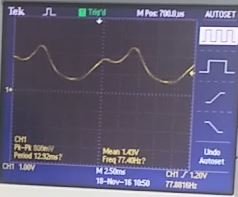
\includegraphics[scale=1]{images/INA/result}
\legend{Source: Authors}
\end{figure}
